\documentclass{article}

% ---- RANDOM FORMATTING ---- %
\setlength{\parindent}{0pt}
%\renewcommand{\thesection}{\Roman{section}} 


% ---- PACKAGES ---- %
\usepackage[margin=2cm]{geometry}
\usepackage{tikz} % graphs
\usepackage{tikz-cd} % commutative diagrams
\usetikzlibrary{decorations.pathreplacing} % for curly braces 
\usetikzlibrary{arrows,shapes,positioning,calc}
\usetikzlibrary{decorations.markings}
\usepackage{amsmath} % ams lot
\usepackage{amsthm} 
\usepackage{amssymb}
\usepackage{parallel}
\usepackage{nicefrac}
\usepackage[normalem]{ulem} % this is for a stupid joke in my Galois representations notes
\usepackage{bbm} % blackboard bold numbers
%\usepackage{mathpazo} % for blackboard bold
%\usepackage{amsfonts}
%\usepackage{mathabx}
%\usepackage{MnSymbol}
%\usepackage{newpxtext} % font
%\usepackage{tgpagella} % font
\usepackage{epigrafica} % font
\usepackage{fourier} % font
%\usepackage{mathptmx} % maths font
%\usepackage{txfonts} % font
\usepackage[bb=ams, cal=cm, scr=rsfs, bbsymbols, calscaled=.96, bbscaled=.96]{mathalpha} % sets the calligraphic to mathcal, scr to rsfs, and blackboard bold to ams
\NewCommandCopy{\pazomathbb}{\mathbb} % if using fourier, this and the line above stop it from using the horrible looking fourier bb font
\AtBeginDocument{\RenewCommandCopy{\mathbb}{\pazomathbb}} % ^
\usepackage{enumerate} % fancy labelling for lists 
% \usepackage{enumitem} % resuming lists - CLASHES WITH ABOVE
\usepackage{pgfplots}
\pgfplotsset{compat=1.18}
\usepgfplotslibrary{fillbetween}
\usepackage{float}
\usepackage{caption} % i do not entirely know -- some latex on stackexchange taught me how to do side-by-side figures
\usepackage{subcaption}
\usepackage[dvipsnames]{xcolor}
\usepackage[most]{tcolorbox} % for fancy boxes
\tcbuselibrary{skins,breakable,theorems} % this is for fancy box formatting
\usepackage{fontawesome}
%\usepackage[sc]{titlesec} % smallcaps section headings
\usepackage{imakeidx} % index generator
\makeindex

\usepackage[hidelinks]{hyperref} % clicky links

% ---- TIKZ ---- %
\usepackage{tikz}

\usetikzlibrary{arrows,shapes,positioning}
\usetikzlibrary{decorations.markings}
\usetikzlibrary{fadings,patterns}

% SNAKE ARROWS STYLE! The argument is the angle
\tikzcdset{snaky/.style={rounded corners,to path={[rotate=#1] -- ($(\tikztostart.#1)+(2ex,0)$)%
 -- ({$(\tikztostart.#1)+(2ex,0)$} |- {$0.5*(\tikztostart)+0.5*(\tikztotarget)$})%
 -- ({$(\tikztotarget.\number\numexpr 180+(#1) \relax)+(-2ex,0)$} |- {$0.5*(\tikztostart)+0.5*(\tikztotarget)$}) \tikztonodes%
 -- ($(\tikztotarget.{\number\numexpr 180+(#1) \relax})+(-2ex,0)$)%
 -- (\tikztotarget)}}}


\tikzstyle arrowstyle=[scale=1]
\tikzstyle directed=[postaction={decorate,decoration={markings, mark=at position .6 with {\arrow[arrowstyle]{stealth}}}}]
\tikzstyle Node=[circle, draw=black, fill=black!10]

\pgfplotsset{compat=1.18}

\hypersetup{colorlinks=true, linkcolor=RedViolet} % sets links to be plum coloured


% ---- COMMANDS ---- %
% mathbb commands
\newcommand{\A}{\mathbb{A}}
\newcommand{\D}{\mathbb{D}}
\newcommand{\R}{\mathbb{R}}
\newcommand{\Q}{\mathbb{Q}}
\newcommand{\Pruf}{\mathbb{D}}
\newcommand{\Z}{\mathbb{Z}}
\newcommand{\N}{\mathbb{N}}
\newcommand{\F}{\mathbb{F}}
\newcommand{\bbG}{\mathbb{G}}
\newcommand{\PP}{\mathbb{P}}
\newcommand{\Hyp}{\mathbb{H}}
\newcommand{\Uni}{\mathbb{U}\mathrm{ni}}
\newcommand{\Gm}{\bbG_{\mathrm{m}}}
\newcommand{\Ga}{\bbG_{\mathrm{a}}}
\newcommand{\triv}{\mathbbm{1}}

% mathcal/mathscr commands
\newcommand{\E}{\mathcal{E}}
\newcommand{\Hopf}{\mathscr{H}}
\newcommand{\GHopf}{\mathscr{G}}
\newcommand{\GLHopf}{\mathscr{G\!l}\!}
\newcommand{\SLHopf}{\mathscr{S\!l}\!}
\newcommand{\inducedop}[2][A]{{#2}_{|_{#1}}}
\newcommand{\ints}{\mathcal{O}}
\newcommand{\Autforms}{\mathcal{A}}
\newcommand{\modforms}{\mathcal{M}}
\newcommand{\cuspforms}{\mathcal{S}}
\newcommand{\Ell}{\mathcal{L}}
\newcommand{\Hilb}{\mathcal{H}}
\newcommand{\calC}{\mathcal{C}}
\newcommand{\calD}{\mathcal{D}}
\newcommand{\calQ}{\mathcal{Q}}
\newcommand{\scrR}{\mathscr{R}}

% mathbf/boldsymbol commands
\newcommand{\Set}{\mathbf{Set}}         % (Set)s
\newcommand{\Grp}{\mathbf{Grp}}         % (Gr)ou(p)s
\newcommand{\Vect}{\mathbf{Vect}}       % (Vect)or spaces
\newcommand{\Mod}{\mathbf{Mod}}         % (Mod)ules
\newcommand{\CRing}{\mathbf{CRing}}     % (C)ommutative (Ring)s
\newcommand{\CAlg}{\mathbf{CAlg}}		% (C)ommutative (Alg)ebras
\newcommand{\Sep}{\mathbf{Sep}}         % (Sep)arable field extensions
\newcommand{\bfrho}{\boldsymbol{\rho}}  % universal deformation
\newcommand{\bfchi}{\boldsymbol{\chi}}  % universal character


% mathrm commands
\newcommand{\Gal}{\mathrm{Gal}} % (Gal)ois group
\newcommand{\Sel}{\mathrm{Sel}} % (Sel)mer group
\newcommand{\Hom}{\mathrm{Hom}} % (Hom)set
\newcommand{\End}{\mathrm{End}} % (End)omorphisms
\newcommand{\Aut}{\mathrm{Aut}} % (Aut)omorphisms
\newcommand{\Frob}{\mathrm{Frob}} % (Frob)enius elements
\newcommand{\Frat}{\mathrm{Frat}} % (Frat)tini quotient
\newcommand{\Rep}{\mathrm{Rep}} % category of (Rep)resentations
\newcommand{\Def}{\mathrm{Def}} % (Def)ormation functor
\newcommand{\DefQ}{\Def_{\calQ}} % (Def)ormation functor with property (Q)
\newcommand{\Irr}{\mathrm{Irr}} % (Irr)educibles
\newcommand{\Isom}{\mathrm{Isom}} % (Isom)etries
\newcommand{\Ext}{\mathrm{Ext}} % (Ext)ensions
\newcommand{\Cl}{\mathrm{Cl}} % (Cl)ass group
\newcommand{\K}{\mathrm{K}} % K theory
\newcommand{\cohom}{\mathrm{H}} % co(H)omology
\newcommand{\res}{\mathrm{res}} % (res)triction
\newcommand{\Res}{\mathrm{Res}} % (Res)triction -- capitalised for rep theory
\newcommand{\cores}{\mathrm{cores}} % (cores)triction
\newcommand{\Ind}{\mathrm{Ind}} % (Ind)uction
\newcommand{\ab}{\mathrm{ab}} % (ab)elianisation
\newcommand{\rad}{\mathrm{R}} % (R)adical (algebraic groups)
\newcommand{\unip}[1]{{#1}_{\mathrm{u}}} % (u)nipotent (subscript)
\newcommand{\uniprad}{\mathrm{R}_{\mathrm{u}}} % unipotent radical
\newcommand{\Pgp}{\mathrm{P}} % P (projection to (P)GL)
\newcommand{\Special}{\mathrm{S}} % S (intersection with (S)L)
\newcommand{\GL}{\mathrm{GL}} % classical groups below
\newcommand{\SL}{\mathrm{SL}}
\newcommand{\PSL}{\Pgp\SL}
\renewcommand{\O}{\mathrm{O}}
\newcommand{\SO}{\mathrm{SO}}
\newcommand{\SU}{\mathrm{SU}}
\newcommand{\Sp}{\mathrm{Sp}}
\newcommand{\Gr}{\mathrm{Gr}} % (Gr)assmannian
\newcommand{\Spec}{\mathrm{Spec}} % Affine scheme
\newcommand{\Spf}{\mathrm{Spf}} % Formal scheme
\newcommand{\Proj}{\mathrm{Proj}} % (Proj)ective affine scheme
\newcommand{\Frac}{\mathrm{Frac}} % Field of (Frac)tions
\newcommand{\ev}{\mathrm{ev}} % (ev)aluation map
\newcommand{\coker}{\mathrm{coker}} % (coker)nel
\newcommand{\im}{\mathrm{im}} % (im)age
\newcommand{\tr}{\mathrm{tr}} % (tr)ace
\newcommand{\lcm}{\mathrm{lcm}} % (l)east (c)ommon (m)ultiple
\newcommand{\trans}{\mathrm{trf}} % (tr)ans(f)er map
\newcommand{\norm}{\mathrm{N}} % (N)orm map
\newcommand{\milnor}{\mathrm{M}} % (M)ilnor (superscript for K-theory)
\newcommand{\nr}{\mathrm{nr}} % u(nr)amified
\newcommand{\et}{\mathrm{\acute{e}t}} % (ét)ale
\newcommand{\Char}{\mathrm{char}} % (char)acteristic of a ring
\newcommand{\Ad}{\mathrm{Ad}} % (Ad)joint representation


% mathfrak commands
\newcommand{\ratfuncs}{\mathfrak{K}}
\newcommand{\Liealg}{\mathfrak{g}}
\newcommand{\eideal}{\mathfrak{e}}
\newcommand{\hyperb}{\mathfrak{H}}
\newcommand{\prid}{\mathfrak{p}}
\newcommand{\mxid}{\mathfrak{m}}
\newcommand{\nxid}{\mathfrak{n}}
\newcommand{\qprid}{\mathfrak{q}}
\newcommand{\Prid}{\mathfrak{P}}
\newcommand{\ideal}{\trianglelefteq}
\newcommand{\id}{\mathrm{id}}
\newcommand{\cl}{\mathrm{cl}}


\newcommand{\mono}{\hookrightarrow}
\newcommand{\epi}{\twoheadrightarrow}
\newcommand{\iso}{\stackrel{\sim}{\smash{\longrightarrow}\rule{0pt}{0.4ex}}}
\newcommand{\To}{\Rightarrow}
\newcommand{\ot}{\leftarrow}
\newcommand{\oT}{\Leftarrow}
\newcommand{\actson}{\circlearrowright}
\makeatletter
\newcommand{\xRightarrow}[2][]{\ext@arrow 0359\Rightarrowfill@{#1}{#2}}
\makeatother

\newcommand{\gen}[1]{\left\langle#1\right\rangle}
\newcommand{\ggen}[1]{\left\langle\!\left\langle #1\right\rangle\!\right\rangle}
\newcommand{\stein}[1]{\left\{ #1 \right\}}
\newcommand{\sstein}[1]{\stein{\!\!\stein{ #1 }\!\!}}
\newcommand{\ssstein}[1]{\stein{\!\!\sstein{-,-}\!\!}}
\newcommand{\sqbrack}[1]{\left[#1\right]}
\newcommand{\ssqbrack}[1]{\left\llbracket#1\right\rrbracket}
\newcommand{\abs}[1]{\left| #1 \right|}
\newcommand{\aabs}[1]{\left|\!\left| #1 \right|\!\right|}

\newcommand{\wt}[1]{\widetilde{#1}}
\newcommand{\wh}[1]{\widehat{#1}}
\newcommand{\ol}[1]{\overline{#1}}
\newcommand{\ul}[1]{\underline{#1}}
\newcommand{\bemph}[1]{\textcolor{RubineRed}{\emph{#1}}}
\newcommand{\smallfrac}[2]{{\textstyle \frac{#1}{#2}}}
\newcommand{\legendre}[2]{\genfrac{(}{)}{}{}{#1}{#2}}


\newcommand{\eps}{\varepsilon}
\newcommand{\quickmatrix}[1]{\begin{pmatrix} #1 \end{pmatrix}}

\newcommand{\congr}{\mathrm{cg}}
\newcommand{\cgsubgp}{\leq_{\congr}}

\newcommand{\ch}{\mathrm{ch}}

\newcommand{\BS}{\mathrm{BS}} % Borel-Serre compact'n
\newcommand{\Exc}{\textcolor{RubineRed}{$\ast$} \textbf{Exc}} % exercise marker

% Defines \Sha
\usepackage[T2A,T1]{fontenc} % the latter two options are for epigrafica (LGR,OT1) -- IF USING FOURIER PACKAGE, DON'T USE OT1
\DeclareSymbolFont{cyrillic}{T2A}{cmr}{m}{n}
\DeclareMathSymbol{\Sha}{\mathalpha}{cyrillic}{216}

% this bit does xleftrightarrow
\makeatletter
\newcommand\xleftrightarrow[2][]{%
  \ext@arrow 9999{\longleftrightarrowfill@}{#1}{#2}}
\newcommand\longleftrightarrowfill@{%
  \arrowfill@\leftarrow\relbar\rightarrow}
\makeatother


\renewcommand{\C}{\mathbb{C}} % these have to be here because fontenc fucks with them
\renewcommand{\U}{\mathrm{U}}
\renewcommand{\mod}[1]{\,\,\mathrm{mod}\,\, #1}

% Source - https://tex.stackexchange.com/a
% Posted by AboAmmar, modified by community. See post 'Timeline' for change history
% Retrieved 2026-01-14, License - CC BY-SA 4.0

%\numberwithin{equation}{section}


% THIS IS SOME LATEX MAGIC THAT LETS YOU REFER TO CUSTOM ITEMIZE LABELS USING HYPERREF
% to use, use \item[\nameditem{ref:erence}{LABEL}] in an itemize environment
% this renders as `LABEL blah blah blah' and is referenced by \ref{ref:erence}
\makeatletter
\def\nameditem#1#2{\begingroup
	#2%
	\def\@currentlabel{#2}%
	\phantomsection\label{#1}\endgroup
}
% Source - https://tex.stackexchange.com/a/730517/432002, Yerasito


% ---- AMSTHM ENVs ---- %
\newcommand{\newmarkedtheorem}[1]{%
  \newenvironment{#1}
	{%
	  \renewcommand{\qedsymbol}{\ensuremath{\diamondsuit}} % this makes the end symbol of an eg into a diamond
	  \pushQED{\qed}\csname inner@#1\endcsname
	}
	{\popQED\csname endinner@#1\endcsname}%
  \newtheorem{inner@#1}%
}

\theoremstyle{definition}
\newtheorem{DEFN}{Definition}[section]
\newtheorem{prop}[DEFN]{Proposition}
\newtheorem{lemma}[DEFN]{Lemma}
\newmarkedtheorem{eg}[DEFN]{Example}
\newmarkedtheorem{noneg}[DEFN]{Non-example}
\newtheorem*{rmk}{Remark}
\newtheorem{cor}{Corollary}[DEFN]
\newtheorem*{redcor}{\textcolor{RubineRed}{Corollary}}

\theoremstyle{plain}
\newtheorem{THM}[DEFN]{Theorem}
%\newtheorem{conj}[DEFN]{Conjecture}
\newtheorem{ax}{Axiom}

% fancy definitions
\newtcolorbox{DEFNbox}{
	sharp corners,
	breakable,
	top=.35cm,
	bottom=.25cm,
	left=.35cm,
	right=.35cm,
	colback=black!5!white,
	boxrule=-1pt,
	leftrule=3pt,
	colframe=blue!40!red,
	before skip=\topsep,
	after skip=\topsep,
	fonttitle=\large\bfseries\sffamily,
	enhanced,
}

\newtcolorbox{THMbox}{
	sharp corners,
	breakable,
	top=.35cm,
	bottom=.25cm,
	left=.35cm,
	right=.35cm,
	colback=black!5!white,
	boxrule=-1pt,
	leftrule=3pt,
	colframe=RubineRed,
	before skip=\topsep,
	after skip=\topsep,
	fonttitle=\large\bfseries\sffamily,
	enhanced,
}

\newtcolorbox{conj}[1]{
	sharp corners,
	breakable,
	boxrule=-1pt,
	colframe=blue!40!white,
	top=.25cm,
    bottom=.25cm,
    left=.35cm,
    right=.35cm,
	leftrule=3pt,
	title=\faQuestionCircleO \,\,\emph{#1},
    fonttitle=\large\bfseries\sffamily,
	enhanced,
	coltitle=white,
	colback=black!5!white,
	attach boxed title to top left={xshift=1pt, yshift=-.1cm},
	boxed title style={colback=blue!40!white, boxrule=-1pt, sharp corners}
}

\newenvironment{defn}{\leavevmode\begin{DEFNbox}\begin{DEFN}\vspace{-.15cm}}{\end{DEFN}\end{DEFNbox}\leavevmode}
\newenvironment{thm}[1][]{\leavevmode\begin{THMbox}\begin{THM}[#1]\vspace{-.15cm}}{\end{THM}\end{THMbox}\leavevmode}

\DeclareMathVersion{normal2} % this is to fix a "too many math alphabets" problem % preamble in separate file

\title{\vspace{-1.5cm}\'Etale Fundamental Groups}
\author{Organised by Matt Byrne}
\date{\today}

\newcommand{\Fib}{\mathrm{Fib}}
\newcommand{\Cov}{\mathbf{Cov}}
\newcommand{\FinCov}{\mathbf{FinCov}}
\newcommand{\Fet}{\mathbf{F\acute{e}t}}

\begin{document}
	\maketitle

	\tableofcontents

	\section*{Boring admin stuff}
	We're meeting every Thursday at 13:00-14:00 in \texttt{J11} Hicks, beginning 8\textsuperscript{th} October. Notes will be updated (hopefully) shortly after each talk, and will be emailed out once they're finished. The main reference is Section 5 of Tam\'as Szamuley's \emph{Galois Groups and Fundamental Groups}.\\

	Per the schedule, the current talk outline is:
	\begin{enumerate}
		\item \hyperref[sec:1_motivation_mark]{Motivation and examples} (Mark)
		\item \hyperref[sec:2_schemes_and_morphisms]{Schemes and morphisms} (Diego, split into two talks for time constraints)
		\item Topological fundamental groups as automorphism groups (Pierre-Louis)
		\item Geometric points and the definition of $\pi_1^{\et}$ (Brais)
		\item \'Etale deck transformations and pro-objects (Matt)
		\item Examples (Matt)
		\item Galois theory for finite \'etale covers (Hao)
		\item Outer Galois actions and further examples (Mark).
	\end{enumerate}

	% sections
	\section{Motivation and examples (Mark)}
\label{sec:1_motivation_mark}
\subsection{Fundamental groups and covers: the classical case}
\label{subsec:1_1_pi1_covers}
Let $X$ be a topological space. One historically important problem is that of classifying the \emph{covering spaces} of $X$.

\begin{defn}
	\label{defn:covering_space}
	Suppose $X$ and $Y$ are topological spaces. A continuous map $p:Y \to X$ is called a \bemph{cover} if for all $x \in X$, there is an open neighbourhood $U_x \subseteq X$ of $x$ whose preimage decomposes as a disjoint union of homeomorphic copies of $U_x$, that is, we may decompose
	\[
		p^{-1} [U_x] = \coprod_{i \in I} V_{x, i}
	\]
	with each $V_{x,i} \subseteq Y$ open and $p|_{V_{x,i}} : V_{x,i} \iso U_x$ a homeomorphism. We say that $Y$ is a \bemph{covering space} for $X$. If $X$ and $Y$ are additionally pointed (i.e. have distinguished basepoints $x_0 \in X, y_0 \in Y$), and the cover $p: (Y, y_0) \to (X, x_0)$ satisfies $p(y_0) = x_0$, we may say that $(Y, y_0)$ is a \bemph{pointed covering space} of $(X, x_0)$.
\end{defn}

These covering spaces of $X$ define a category $\Cov(X)$, whose morphisms are continuous maps $Y_1 \to Y_2$ commuting with the covers $p_i : Y_i \to X$. We will write $\FinCov(X)$ for the full subcategory of finite covers, and $\Cov_*(X, x_0)$ for the subcategory of pointed covers (with pointed morphisms). \\

One notable property of covering spaces is the \emph{homotopy lifting property}: that given a homotopy $\{f_t :Z \to X\}_{t \in [0,1]}$ of maps to $X$, and a lift $g_0:Z\to Y$ of $f_0$ through $p: Y \to X$, there exists a unique homotopy $\{\hat{f}_t : Z \to Y\}_{t \in [0,1]}$ lifting $\{f_t\}_t$ through $p: Y \to X$ such that $\hat{f}_0 = g_0$. \\

As a consequence of the homotopy lifting property, their fibres admit a \emph{monodromy action}: given a cover $p: Y \to X$ and some $x_0 \in X$, the fibre $p^{-1}(x_0) \subseteq Y$ is a discrete subspace. Given a point $y \in p^{-1}(x_0)$ and some class $[\alpha] \in \pi_1 (X, x_0)$, which we recall is a strong homotopy equivalence class of loops in $X$ based at $x_0$, any representative $\alpha : [0,1] \to X$ lifts to a unique $\hat{\alpha}_y:[0,1] \to Y$ starting at $y$ whose strong homotopy class depends only on the strong homotopy class $[\alpha]$. Thus the endpoint $\hat{\alpha}_y(1)$ does not depend on the choice of lift, and we define $[\alpha] \cdot y := \hat{\alpha}_y(1)$. \\

So we can think of the taking the fibre at $x_0$ as a functor 
\[
	\Fib_{x_0} : \Cov(X) \to \pi_1(X, x_0)\textrm{-}\Set
\]
from the category of covering spaces of $X$ to the category of $\pi_1(X,x_0)$-sets, i.e. discrete sets with an action of $\pi_1(X, x_0)$. As it turns out, when $X$ is especially nice (path-connected, locally path-connected, and semilocally simply connected) this is a \emph{representable functor}, insomuchas 
\[
	\Fib_{x_0}(Y) \cong \Hom_{\Cov(X)}(\tilde{X}, Y)
\]
for some $\tilde{X} \in \Cov(X)$ unique up to isomorphism. Such $\tilde{X}$ is called a \bemph{universal covering space} for $X$, and may be constructed explicitly by choosing a basepoint $x_0 \in X$ and defining
\[
	\tilde{X}_{x_0} := \frac{\{\gamma : [0,1] \xrightarrow{\textrm{cts}} X \mid \gamma(0)=x_0\}}{\mathrm{homotopy}},\qquad \tilde{p} : \tilde{X}_{x_0} \to X;\,\, \gamma \mapsto \gamma(1).
\]
By definition, we see that $\Fib_{x_0}(\tilde{X}_{x_0}) = \pi_1 (X, x_0)$, and thus by universality we see 
\[
	\pi_1(X, x_0) \cong \Hom_{\Cov(X)}(\tilde{X}_{x_0}, \tilde{X}_{x_0}) = \Aut_{\Cov(X)}(\tilde{X}_{x_0})
\]
This final isomorphism is sometimes referred to as the \bemph{deck transformation construction}.

\begin{thm}
	\label{thm:galois_for_covers}
	Pointed covers of a path-connected, locally path-connected, and semilocally simply connected pointed space $(X, x_0)$ are in bijection with subgroups of $\pi_1(X, x_0)$. To each $H \leq \pi_1(X, x_0)$ we associate $(\tilde{X}_{x_0} / H, Hx_0)$, and to each $p:(Y, y_0) \to (X, x_0)$ we associate $p_* \pi_1(Y, y_0) \leq \pi_1(X, x_0)$.
\end{thm}

The main idea of this reading group will be to define a sort of covering space theory for schemes, by way of the \emph{\'etale fundamental group}. But how do we do this?

% double page thing here

\begin{center}
	\begin{tabular}{c|c}
		\textbf{Topological spaces} & \textbf{Schemes}\\
		\hline
		$X$ a nice topological space & $S$ a nice scheme\\
		$p : Y \to X$ a topological cover & $\phi : X \to S$ a \bemph{finite \'etale cover}\\ 
		$x_0 \in X$ a point & $\overline{s_0} : \Spec(\Omega) \to S$ a \bemph{geometric point}\\
		$\pi_1(X, x_0)$ defined in terms of loops/paths & Paths are meaningless in Zariski!\\
		$\pi_1(X,x_0) = \Aut(\Fib_{x_0})$ & $\pi_1^{\et}(S, \overline{s_0})=\Aut(\Fib_{\ol{s_0}})$ \\
		$\tilde{X} \to X$ universal cover (generally infinite degree) & $\mathfrak{X} \in \mathrm{pro}(\Fet_S)$ a \bemph{universal pro-object}\\
		$\pi_1(X, x_0) \cong \Aut(\tilde{X})$ & $\pi_1^{\et}(S, s_0) \cong \varprojlim_{X \in \mathfrak{X}}\Aut(X)$
	\end{tabular}
\end{center}

\leavevmode\\

In fact for complex affine varieties $X_{/ \C}$ we will be able able to define both the classical fundamental group $\pi_1(X^\mathrm{an}, x_0)$ (considering its complex points $X(\C)$ canonically retopologised as a complex manifold $X^\mathrm{an}$) and the \'etale fundamental group $\pi_1^{\et}(X, \overline{x_0})$ (considering it as a scheme, where $\overline{x_0}$ is the geometric point induced by $x_0$), and in this case the two \emph{almost} coincide:
\[
	\pi_1^{\et}(X, \overline{x_0}) \cong \widehat{\pi_1}(X^\mathrm{an}, x_0),
\]
where the only difference is a profinite completion on the right, appearing since we are only considering \emph{finite} covers as we will see later. \\

The approach we will take is to use this recontextualisation of $\pi_1(X, x_0)$ as an automorphism group as the basis for our definition of $\pi_1^{\et}$. After defining all of the scheme theory we will need, we will try to reformulate the theory of covering spaces independent of loops so we can do it for schemes. There will be some interesting differences which will be explained in future talks.

\subsection{An interesting coincidence}
\label{subsec:1_2_Weil_rosetta_stone}
One slightly more specific example which might motivate the need for a theory of \'etale covering space is the famous \emph{Weil Rosetta stone}. This is a set of strange coincidences between the theories of Riemann surfaces and of number fields that seem to suggest that both are offshoots of a more general theory (which will turn out to be our theory of the \'etale fundamental group). To state this, we first must define some things. We will start with the number fields setting.

\subsubsection{A little bit of number theory}
\label{subsubsec:1_2_1_number_fields}
\begin{defn}
	A \bemph{number field} $K$ is a finite field extension of $\Q$. That is, it is a field containing $\Q$ which is finite-dimensional as a $\Q$-vector space. Each number field $K$ admits a distinguished subring $\ints_K$ called its \bemph{ring of integers}, which is the integral closure of $\Z$ in $K$.
\end{defn}

In each extension $L/K$ of number fields, we can look at prime ideals $\prid$ of the ring of integers $\ints_K$ of $K$ (which we be called `primes of $K$' for short). Each such prime must factorise in $\ints_L$ as a unique product 
\[
	\prid\ints_L = \Prid_1^{e_1} \cdots \Prid_r^{e_r}
\]
of powers of primes $\Prid_i$ of $L$. We say that $\prid$ \bemph{ramifies} in $L/K$ if any of the $e_i > 1$, otherwise we say it is \bemph{unramified}.

\begin{eg}
	In the extension $\Q(i)/\Q$, the ideal $5\Z[i]$ factorises as $\gen{2+i}\gen{2-i}$, so $5$ is unramified. In contrast, the ideal $2 \Z[i]$ factorises as $\gen{1+i}^2$ since $(1+i)(1-i)=2$, so $2$ ramifies. 
\end{eg}

If a set $S$ of primes of $K$ contains all of the primes at which $L/K$ ramifies, we say that $L/K$ is \bemph{unramified away from $S$}, or just \bemph{$S$-unramified}.\\ 

Given an algebraic closure $\ol{K}/K$, we can form the \bemph{maximal $S$-unramified extension} $K_S /K$ by taking the union of all finite subextensions $L/K$ of $\ol{K}/K$ which are $S$-unramified. Then we define the \bemph{$S$-unramified absolute Galois group} $G_{K, S}$ to be topological group
\[
	G_{K, S} := \Gal(K_S/K) := \varprojlim_{L / K} \Aut_K(L)
\]
where $L/K$ ranges over all finite, $S$-unramified extensions.

\begin{thm}
	The open subgroups of $G_{K,S}$ are in bijection with the set of finite, $S$-unramified extensions of $K$ contained in $\ol{K}$. An open subgroup $H$ is sent to its fixed field $K_S^H$, and a finite $S$-unramified extension $L/K$ is sent to the open subgroup $\Gal(K_S/L)$.
\end{thm}

There is an underlying geometric object here, called $\Spec(\ints_{K,S})$ (see next week's talk). We will see that finite $S$-unramified extensions correspond to finite \'etale covers $X \epi \Spec(\ints_{K,S})$, and a choice of algebraic closure $\ol{K}$ corresponds to a choice of \emph{geometric basepoint} $\Spec(\ol{K})$.


\subsubsection{A little bit of complex geometry}
\label{subsubsec:1_2_2_riemann_surfaces}
\begin{defn}
	A \bemph{Riemann surface} is a smooth complex manifold of dimension 1.
\end{defn}

We are interested in holomorphic maps between compact Riemann surfaces, so fix a surjective holomorphic map $\phi : Y \to X$. Interestingly, any such map is a finite topological cover away from a finite set of points of $X$, which are called the \bemph{ramification points} of $\phi$. If a discrete subset $S \subset X$ contains all of the ramification points of $\phi$, we say that $\phi$ is \bemph{unramified away from $S$}. \\


Since any finite cover of Riemann surface is itself a Riemann surface, Theorem \ref{thm:galois_for_covers} specialises in this case to give a specific correspondence between pointed, $S$-unramified holomorphic covers of $(X,x_0)$ and finite-index subgroups of $\pi_1(X\setminus S, x_0)$, which is equivalent to the following statement about the profinite completion $\widehat{\pi_1}$ of the fundamental group.

\begin{thm}
	The open subgroups of $\widehat{\pi_1}(X\setminus S, x_0)$ are in bijection with finite, $S$-unramified, pointed holomorphic covers of $(X, x_0)$. An open subgroup $H$ is sent to the compactification of the orbit space $\widetilde{X \setminus S}_{x_0}/H$ with basepoint $Hx_0$, and a finite, $S$-unramified, pointed holomorphic cover $\phi : (Y, y_0) \to (X, x_0)$ is sent to the open subgroup
	\[
		\phi_* \widehat{\pi_1}(Y\setminus \phi^{-1}[S], y_0) \subseteq \widehat{\pi_1}(X\setminus S, x_0).
	\]
\end{thm}

There is an underlying algebraic object here, that being the field $K(X)$ of meromorphic functions on $X$, and the subring $\ints_{X,S}$ of meromorphic functions which are holomorphic away from $S$. Any holomorphic cover $\phi : Y \to X$  realises a field extension $\phi^* : K(X) \mono K(Y)$, and it sends $\ints_{X, S}$ to $\ints_{Y, \phi^{-1}[S]}$.


\subsubsection{Weil's Rosetta stone}
\label{subsubsec:1_2_3_rosetta_stone}
We can formalise this correspondence later, but for now there's a long list of things that seem to be similar. We will write the objects of interest, as well as what the `\'etale equivalent' will be.
\begin{center}
	\begin{tabular}{c|c|c}
		\textbf{Compact Riemann surface} $X$ & \textbf{Number field} $K$ & \emph{\'Etale equivalent} \\
		\hline
		$X$ & & $\Spec(\ints_K)$ \\
		$X'$ &  & $\Spec(\ints_{K,S})$ \\
		$\phi : Y \epi X$ holomorphic & $\iota : K \mono L$ finite extension & $\iota^* : \Spec(\ints_L) \epi \Spec(\ints_K)$ finite smooth \\
		$S$ ramification points & $S$ ramified primes & $S$ ramification points \\
		$\phi$ is $S$-unramified  & $L/K$ is $S$-unramified & $\iota^*$ is $S$-unramified\\
		$\phi|_{Y'} \in \FinCov(X\setminus S)$ & & $\iota^*|_{\Spec(\ints_{L,S})} \in \Fet(\Spec(\ints_{K,S}))$ \\
		$x_0 \in X'$ basepoint & $\ol{K}/K_S/K$ algebraic closure & $\overline{s_0}:\Spec(\ol{K}) \to \Spec(\ints_{K,S})$ geom. point \\
		$\widehat{\pi_1}(X', x_0)$ & $G_{K,S}:=\Gal(K_S/K)$ & $\pi_1^{\et}(\Spec(\ints_{K,S}), \overline{s_0})$ \\
		$\phi^{-1}(x)$ & Primes above $\prid \notin S$ & $\Spec(\ints_{L,S}) \times_{\Spec(\ints_{K,S})} \Spec(\Omega)$\\
		Classification of hol. covers & Galois theory & Still to come...
	\end{tabular}
\end{center}

Here we write $X' := X \setminus S$ and $Y' := Y \setminus \phi^{-1}[S]$ for brevity's sake.

\subsubsection{A bonus "rad" fact}
Though not entirely in the spirit of finite \'etale covers, the analogy between compact Riemann surfaces and number fields is even deeper than this. This subsection is only included for fun and is very informal, so feel free to skip it!\\

One of the greatest achievements of early 20\textsuperscript{th} Century number theory was the development of \emph{class field theory}. The point of class field theory is to classify every so-called abelian number field, i.e. number fields with abelian Galois group over $\Q$. Along with the development of a theory of analysis over $\Q$ (i.e. analysis over the ring $\A_\Q$ of ad\`eles of $\Q$), it is known for some fairly mysterious isomorphisms. One of the most notable being:
\[
	G_{K, S}^{\ab} \cong K^\times \backslash \A_{K, \mathrm{fin}}^\times / U_S,\qquad U_S:= \prod_{v \notin S} U_v.
\]
The double quotient group here may be thought of as the Picard group of $\Spec(\ints_{K,S})$, i.e. we may think of this as a canonical isomorphism 
\[
	G_{K,S}^{\ab} \cong \mathrm{Pic}(\Spec\,\ints_{K,S}).
\]
Simultaenously on the other side, if we take the (punctured) compact Riemann surface $X' := X\setminus S$ we may consider its \emph{Jacobian variety}
\[
	\mathrm{Jac}(X') := H^0(X', \Omega_{X'}^1)^* / H_1(X')
\]
where a 1-chain $\gamma$ is seen as a functional on global holomorphic differentials via the usual pairing $(\gamma, \omega) \mapsto \int_\gamma \omega$. Then \emph{geometric class field theory} gives another mysterious canonical isomorphism 
\[
	\pi_1(X', x_0)^{\ab} \otimes \R/\Z \cong \mathrm{Jac}(X').
\]
Since $\mathrm{Jac}(X')$ may be seen as the identity component of the Picard variety, Weil's Rosetta stone suggests that these two statements are somewhat analogous. Writing $Z' := \Spec(\ints_{K,S})$ and $\overline{z_0} : \Spec(\ol{K}) \to Z'$, the statements even kind of looks the same:
\[
	\pi_1^{\et}(Z', \ol{z_0})^{\ab} \cong \mathrm{Pic}(Z') \,\,\Longleftrightarrow\,\, \pi_1(X', x_0)^{\ab} \otimes \R/\Z \cong \mathrm{Pic}^\circ (X').
\]
Perhaps the most interesting thing here, however, is why these statements are different. Why the extra $\R/\Z$? Why $\pi_1$ instead of $\widehat{\pi_1}=\pi_1^{\et}$? Why $\mathrm{Jac}=\mathrm{Pic}^\circ$ instead of $\mathrm{Pic}$? The answers to these questions are simple... I don't know. But we may find out in one of the bonus lectures! 		% section 1 	-- motivation + examples
	\section{Schemes and morphisms (Diego)} % Diego's talk(s)
\label{sec:2_schemes_and_morphisms}
\subsection{Some classical algebraic geometry}
\label{subsec:2_1_classical_AG}
How much can we know about spaces from their functions? A simple example here is the space $\C^n$. Consider the set $R$ of polynomial functions $\C^n \to \C$, which may be identified as $R=\C[x_1, \ldots, x_n]$. Then for each point $p = (p_1, \ldots, p_n) \in \C^n$, we may define the evaluation map $\ev_p : R \to \C$ given by $\ev_p(f) := f(p)$. Clearly this is a surjective morphism of $\C$-algebras, so we can think of this as a map quotienting out by the maximal ideal 
\[
	\mxid_p := \ker(\ev_p) = (x_1-p_1,\ldots,x_n-p_n).
\] 
In fact, all maximal ideals of $R$ are of the form $\mxid_q$ for some $q \in \C^n$, so this defines a bijection
\[
	\begin{tikzcd}[row sep=tiny]
		\C^n \ar[r, leftrightarrow, "\sim"] & \Spec_\mxid(R) \\
		p \rar[mapsto] & \mxid_p 
	\end{tikzcd}
\]
where $\Spec_\mxid(R)$ denotes the \bemph{maximal spectrum} of $R$, that is, the set of maximal ideals of $R$. For each subset $U \subseteq \C^n$ and ideal $J \ideal R$, we may then extend this construction by defining 
\[
	\I(U) := \bigcap_{p \in U} \mxid_p, \quad \text{and} \quad \V(J) := \{p \in \C^n \mid \forall f \in J, \, f(p) = 0 \}.
\]
These two maps end up to be inclusion reversing, and thus define an antitone Galois connection
% https://q.uiver.app/#q=WzAsMixbMCwwLCJcXGxlZnRcXHsgXFxzdWJzdGFja3tcXHRleHR7U3Vic2V0c31cXFxcXFx0ZXh0e29mIH1cXENebn0gXFxyaWdodFxcfSJdLFsyLDAsIlxcbGVmdFxceyAgXFxzdWJzdGFja3tcXHRleHR7SWRlYWxzfSBcXFxcIFxcdGV4dHtvZiB9Un0gXFxyaWdodFxcfSJdLFswLDEsIkkiLDAseyJjdXJ2ZSI6LTJ9XSxbMSwwLCJWIiwwLHsiY3VydmUiOi0yfV1d
\[\begin{tikzcd}
	\begin{array}{c} \left\{ \bettersubstack{\text{Subsets}\\\text{of }\C^n} \right\} \end{array} && \begin{array}{c} \left\{  \bettersubstack{\text{Ideals} \\ \text{of }R} \right\} \end{array}
	\arrow["\I", curve={height=-12pt}, from=1-1, to=1-3]
	\arrow["\V", curve={height=-12pt}, from=1-3, to=1-1]
\end{tikzcd}\]
which restrict to inclusion reversing bijections between the \emph{radical ideals} of $R$ (i.e. those such that if $x^n \in J$ then $x \in J$), and the so-called \emph{algebraic sets} (this is \emph{Hilbert's Nullstellensatz}).

\begin{defn}
	A subset $X \subseteq \C^n$ is called an \bemph{algebraic subset} if it is defined to be the common zero locus of a set of $n$-variable polynomials in $\C^n$.
\end{defn}

We note that:
\begin{itemize}
	\item $\C^n = \V(0)$, so $\C^n$ is an algebraic subset of itself;
	\item $\varnothing = \V(1)$, so $\varnothing$ is an algebraic subset of itself;
	\item as a consequence of \emph{Hilbert's Basis Theorem} (i.e. that $R$ is Noetherian), arbitrary intersections of algebraic subsets are algebraic; and
	\item as a consequence of the fact $\V(f) \cup \V(g) = \V(fg)$, finite unions of algebraic subsets are algebraic.
\end{itemize}
All of these properties say that the algebraic subsets define the closed sets of a topology on $\C^n$, which we call the \bemph{Zariski topology} $\mathcal{T}_\text{Zar}$. That is, a subset of $\C^n$ is Zariski-closed if and only if it is algebraic. 

\begin{defn}
	When $\C^n$ (or equivalently, $k^n$ for a field $k$) is endowed with the Zariski topology $\mathcal{T}_\text{Zar}$, it is referred to as (complex) \bemph{affine $n$-space} $\A^n$. A Zariski closed subset of $\A^n$ endowed with the subspace topology is referred to as a (complex) \bemph{closed affine algebraic variety} (or just a \emph{CAAV}).
\end{defn}

We can check that a basis for the open sets of the Zariski topology is given by open sets of the form
\[
	D_f := \{p \in \A^n \mid f(p) \neq 0\},
\]
which are huge for nonzero polynomials $f\in R$ (cf. Figure \ref{fig:zariski_open})! Because of this, CAAVs are very poorly behaved topological spaces (e.g. they're not Hausdorff), so continuous maps should not necessarily be our notion of a `nice' map. We are usually more interested in polynomial functions on these spaces, which preserve this algebraic structure.

\begin{figure}[H]
	\centering
	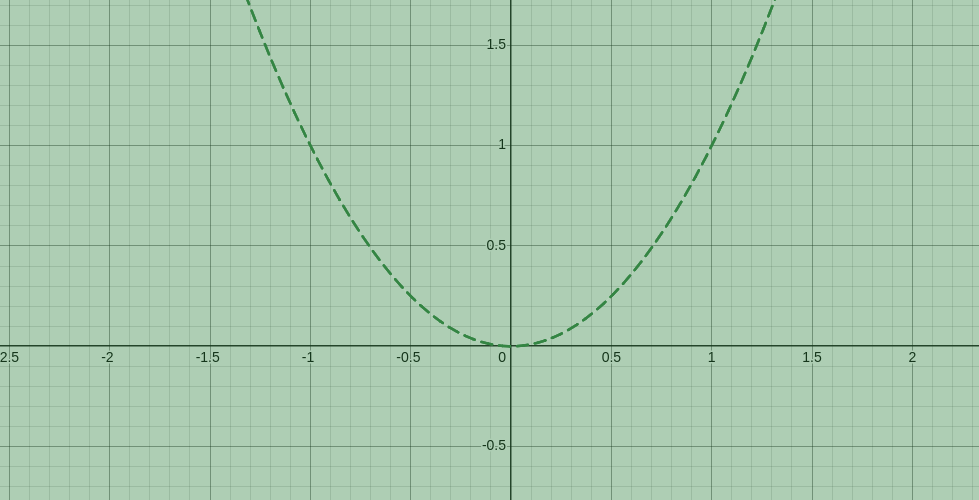
\includegraphics[width=0.5\textwidth]{Images/zariski_open.png}
	\caption{The basic open set $D_{y-x^2}$ in $\A^2$ shaded in light green.}
	\label{fig:zariski_open}
\end{figure}

\begin{eg}
	Let $X = \V(x^2 + y^2 - 1) \subseteq \A^2$ be the circle in the plane\footnote{While we are usually considering things over $\C$, which has topological dimension 2, the algebraic dimension of affine $n$-space is $n$ and so $\A^1$ is referred to as \emph{the line}, $\A^2$ as \emph{the plane}, etc.}. What would the polynomial functions $X \to \A^1$ even be? Well, these should be the restriction of a polynomial function $\A^2 \to \A^1$ to $X$, considered equal if and only if they agree at all points of $X$. The polynomial functions $\A^2 \to \A^1$ are just 2-variable complex polynomials, $\C[x,y]$, and two polynomials $f, g \in \C[x,y]$ agree on $X$ if and only their difference $f-g$ is zero on $X$. The polynomials which are zero on $X$, by definition, are the elements of the vanishing ideal $\I(X) = (x^2 + y^2 - 1)$, and so the polynomial functions $X \to \A^1$ may be identified with elements of the quotient $\C[x, y]/(x^2 + y^2 - 1)$.
\end{eg}

\begin{defn}
	For a closed affine algebraic variety $X \subseteq \A^n$, its \bemph{coordinate ring} $\ints(X)$ is the ring of polynomial functions $X \to \A^1$, that is, it is the quotient ring 
	\[
		\ints(X) := \frac{\C[x_1,\ldots,x_n]}{\I(X)}.
	\]
\end{defn}

We note a few things about coordinate rings of CAAVs over $\C$:
\begin{itemize}
	\item the coordinate ring $\ints(X)$ is a $\C$-algebra, since constant functions are polynomial;
	\item since $\I(X)$ is radical and $\C[x_1, \ldots, x_n]$ is an ID, the quotient $\ints(X)$ is \emph{reduced} (it has no nilpotents);
	\item since $\C[x_1, \ldots, x_n]$ is Noetherian and finitely-generated as a $\C$-algebra, $\ints(X)$ is finitely-generated as a $\C$-algebra.
\end{itemize}

This association of a coordinate ring to each CAAV over $\C$ may be seen to give an equivalence of categories
\[
	\begin{tikzcd}
		\left\{\bettersubstack{\text{closed, affine,} \\ \text{algebraic varieties} \\ \text{over }\C}\right\} \rar[leftrightarrow, "\simeq"] & \left\{\bettersubstack{\text{finitely generated,}\\ \text{reduced, commutative} \\ \C\text{-algebras}}\right\}^{\text{op}}
	\end{tikzcd}
\]
The fully-faithful property is pretty easy to see (our morphisms of CAAVs are just polynomial maps), but the essential surjectivity on objects is a bit more tricky. To show this we think back to the observation that at the beginning of the chapter that points of $\A^n$ are in bijection with maximal ideals of $\C[x_1, \ldots, x_n]$.\\ 

It is not too hard to show that this also holds of any complex CAAV $X$: that points of $X$ are in bijection with maximal ideals of $\ints(X)$. So if we endow $\Spec_\mxid(\ints(X))$ with the Zariski topology, we can view the maximal spectrum \emph{itself} as a CAAV.\\ 

To do this we only need to recall that the evaluation map $\ev_p$ may be seen as the quotient by $\mxid_p$, so the `evaluation' of a `function' $f \in \ints(X)$ at a `point' $\mxid_1 \in \Spec_\mxid(\ints(X))$ is defined to be the residue class $f \mod{\mxid}$. Translating the definition of the basic open sets of $X$ into this language, a basis for the Zariski topology on $\Spec_\mxid (\ints(X))$ is given by the sets of the form 
\[
	D_f := \{ \mxid_1 \in \Spec_\mxid(\ints(X)) \mid f \notin \mxid_1 \}.
\]
Given a finitely generated, reduced, commutative $\C$-algebra $A$, its maximal spectrum $\Spec_\mxid(A)$ under the Zariski topology may then be seen as a closed affine algebraic variety over $\C$ whose coordinate ring is $A$, giving essential surjectivity. To repeat, 
\begin{center}
	a closed affine algebraic variety $X$ \textbf{is} the maximal\\spectrum of its coordinate ring $\ints(X)$:
	\[
		X = \Spec_\mxid(\ints(X))
	\]
\end{center}
As for why this is functorial, the morphism of CAAVs corresponding to an algebra homomorphism $\varphi : A \to B$ is 
\[
	\Spec_\mxid(\varphi) : \Spec_\mxid(B) \to \Spec_\mxid(A), \qquad \mxid_B \mapsto  \phi^{-1}(\mxid_B).
\]


\subsubsection{Why move to schemes?}
\label{subsubsec:2_1_1_why_schemes}
\begin{itemize}
	\item We want to create a similar theory that accepts \emph{any} commutative ring, rather than exclusively finitely generated, reduced, commutative $\C$-algebras;
	\item Since algebraic subsets correspond to radical ideals, this theory does not see points with multiplicity/rings with nilpotence. For example, the equation $x^2 =0$ in $\A^1$ should correspond to a point at zero \emph{with multiplicity 2}, but $\V(x^2) = \V(\sqrt{(x^2)}) = \V(x)$ which only sees that there is a point at zero and forgets the multiplicity;
	\item While $\Spec_\mxid$ is functorial for our FGRC $\C$-algebras, it fails to be functorial in general (preimages of maximal ideals under general ring homomorphisms are rarely maximal, e.g. $(0)$ in $\Z \to \Q$). 
\end{itemize}

\subsection{Affine schemes}
\label{subsec:2_2_affine_schemes}
In much the same way that the theory of varieties revolves around the maximal spectrum, the theory of schemes is based on the \bemph{spectrum} of a commutative ring $R$. This is the set of \emph{prime} ideals of $R$, which we also endow with the Zariski topology 
\[
	\Spec(R) = \{\prid \ideal R \ \text{prime}\}, \qquad D_f = \{\prid \in \Spec(R) \mid f \notin \prid\}, \qquad \mathcal{T}_\text{Zar} = \gen{D_f \mid f \in R}.
\]

For simplicity, we will assume from now on that all rings $R$ are integral domains unless otherwise specified, but bear in mind that all of this can be done over non-integral domains (the definition of localisation does change in this case though).

\begin{defn}
	An \bemph{affine scheme} is a pair $(X, \ints_X)$, where $X = \Spec(R)$ for some commutative ring $R$, and $\ints_X$ is a sheaf\footnote{If you don't know what a sheaf is, I've included \hyperref[appendix:A_sheaves]{a short appendix} on everything you'll need to know about them.} on $X$ (called the \bemph{structure sheaf}) defined on the basic Zariski-open sets $D_f$ to be the localisation of $R$ at $f$
	\[
		\ints_X (D_f) := R_f = R\left[\frac{1}{f}\right],
	\]
	i.e. those elements of the field of fractions $\Frac(R)$ of the form $g / f^n$, where $g \in R$ and $n \in \Z$. The restriction morphisms $\res:\ints_X(D_f) \to \ints_X(D_{fg})$ is the usual inclusion map.
\end{defn}

We can check that the stalks of $\ints_X$ are given by
\[
	\ints_{X, \prid} = \varinjlim_{U \ni \prid} \ints_X(U) = R_\prid,
\]
the localisation of $R$ at $\prid$, i.e. those elements of $\Frac(R)$ whose denominator is not in $\prid$. Since $R_{\prid}$ is local, affine schemes are locally ringed spaces. If a locally ringed space $(X, \ints)$ is isomorphic to an affine scheme, we will call it an affine scheme also.\\

As before, for each $\prid \in \Spec(R)$ we define the \bemph{evaluation map} $\ev_\prid$ to be the quotient map with kernel $\prid$, although now it is valued in the \bemph{residue field} $k(\prid) := \Frac(R/\prid) = R_\prid / \prid R_\prid$. This allows us to define our $\V$ and $\I$ functions as before:
\begin{align*}
	\V(J) &:= \{\prid \in \Spec(R) \mid \ev_\prid(f)=0, \ \forall f \in J\} = \{\prid \in \Spec(R) \mid J \subseteq \prid\},\\
	\I(U) &:= \{f \in R \mid \ev_\prid(f) = 0, \ \forall \prid \in U\} = \bigcap_{\prid \in U} \prid,
\end{align*}
where $J\ideal R$ is an ideal and $U \subseteq \Spec(R)$ is a subset. Notably, we see that:
\begin{itemize}
	\item the Zariski-closure $\ol{U}$ of a subset $U \subseteq \Spec(R)$ is exactly $\ol{U} = \V\I(U)$;
	\item the correspondence theorem ensures that $\V(J) \subseteq \Spec(R)$ may be identified with the affine scheme $\Spec(R/J)$, so the Zariski-closed subsets are the spectra of quotients of $R$ (and $\varnothing$);
	\item properties of localisation ensure that $D_f \subseteq \Spec(R)$ may be identified with the affine scheme $\Spec(R_f)$, so the basic Zariski-open subsets are the spectra of localisations of $R$.
\end{itemize}

\begin{eg}
	\begin{enumerate}[(i)]
		\item While we have seen that the closed affine algebraic variety $\Spec_\mxid(\C[x,y])$ may be identified with $\C^n$ under the Zariski topology, we instead look at the prime spectrum $\Spec(\C[x,y])$. As a set, this decomposes as 
			\[
				\Spec(\C[x,y]) = \Spec_\mxid (\C[x,y]) \,\, \cup \,\, \{(0)\} \,\, \cup \,\, \{(f) \mid f \in \C[x,y] \text{ irr.}\}.
			\]
			These different categories of points are distinguished by the Zariski closures of their corresponding singletons, which is exactly $\V\I(\{\prid\})=\V(\prid)$.
			\begin{itemize}
				\item For a point $\mxid_1 \in \Spec_\mxid(\C[x,y])$, i.e. a maximal ideal of $\C[x,y]$, we see that $\ol{\{\mxid_1\}} = \V(\mxid_1)$ is the set of prime ideals containing $\mxid_1$, which is exactly the singleton $\{\mxid_1\}$ since $\mxid_1$ is maximal. For this reason, maximal ideals of $\C[x,y]$ correspond to \bemph{closed points} of $\Spec(\C[x,y])$ (and this works for general rings!);
				\item The point $(0) \in \Spec(\C[x,y])$, i.e. the zero ideal, has $\ol{\{(0)\}} = \V(0) = \Spec(\C[x,y])$. For this reason, the point $(0)$ is called a \bemph{dense point} or a \bemph{generic point} of $\Spec(\C[x,y])$ (and again, this works for general rings);
				\item A point $(f) \in \Spec(\C[x,y])$ with $f \in \C[x,y]$ irreducible has $\ol{\{(f)\}} = \V(f) = \Spec(R/(f))$, which is a closed affine subscheme (i.e. a Zariski closed subset). Such points are thus the generic points of closed affine subschemes of $\Spec(\C[x,y])$.
			\end{itemize}
			So the points of $\Spec(\C[x,y])$ may be thought of as
			\[
				\Spec(\C[x,y]) = \left\{\bettersubstack{\text{closed} \\ \text{points}}\right\} \,\, \cup \,\, \left\{\bettersubstack{\text{generic} \\ \text{point}}\right\} \,\, \cup \,\, \left\{\bettersubstack{\text{generic points of} \\ \text{closed subschemes}}\right\}
			\]
			We may think of generic points as a sort of `codimension 0 point', which is close to everything. 
		\item The affine scheme $\Spec(\C[x]/(x^2))$ decomposes as
			\[
				\Spec\left(\frac{\C[x]}{(x^2)}\right) = \{(x)\} \,\,\cup\,\, \{(0)\}
			\]
			which is just the one closed point, along with the generic point. This is seen to be different to $\Spec(\C[x]/(x)) = \Spec(\C)$, which consists solely of a generic point. So our notion is tracking multiplicity correctly!
		\item One interesting example that may motivate something later: if we consider the prime spectrum of $\Z$, this may be visualised as a long line (corresponding to the generic point) connecting infinitely many points (corresponding to the closed points, the ideals $p\Z$), as in Figure \ref{fig:SpecZ}.
		\begin{figure}[H]
			\centering
			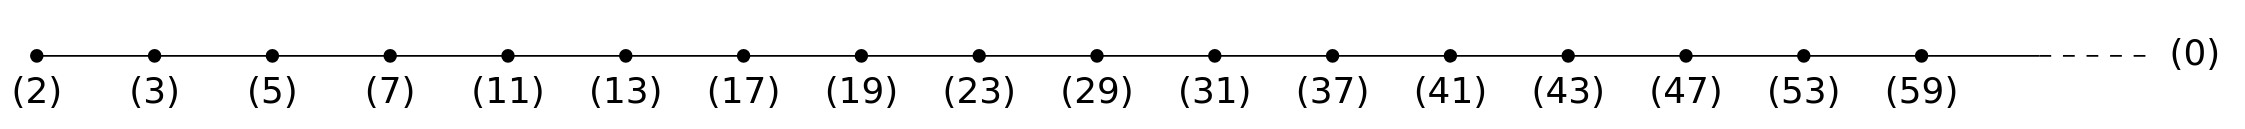
\includegraphics[width=0.7\textwidth]{Images/Spec(Z).png}
			\caption{$\Spec(\Z)$, per the \href{https://www.lmfdb.org/NumberField/1.1.1.1}{LMFDB}.}
			\label{fig:SpecZ}
		\end{figure}
		The inclusion $\Z \mono \Z[\!\sqrt{3}]$ gives us a corresponding surjective morphism $\Spec(\!\Z[\sqrt{3}]) \epi \Spec(\Z)$ which may be visualised as in Figure \ref{fig:SpecZsqrt3_over_SpecZ}, where the vertical columns are the fibres of the morphism.
		\begin{figure}[H]
			\centering
			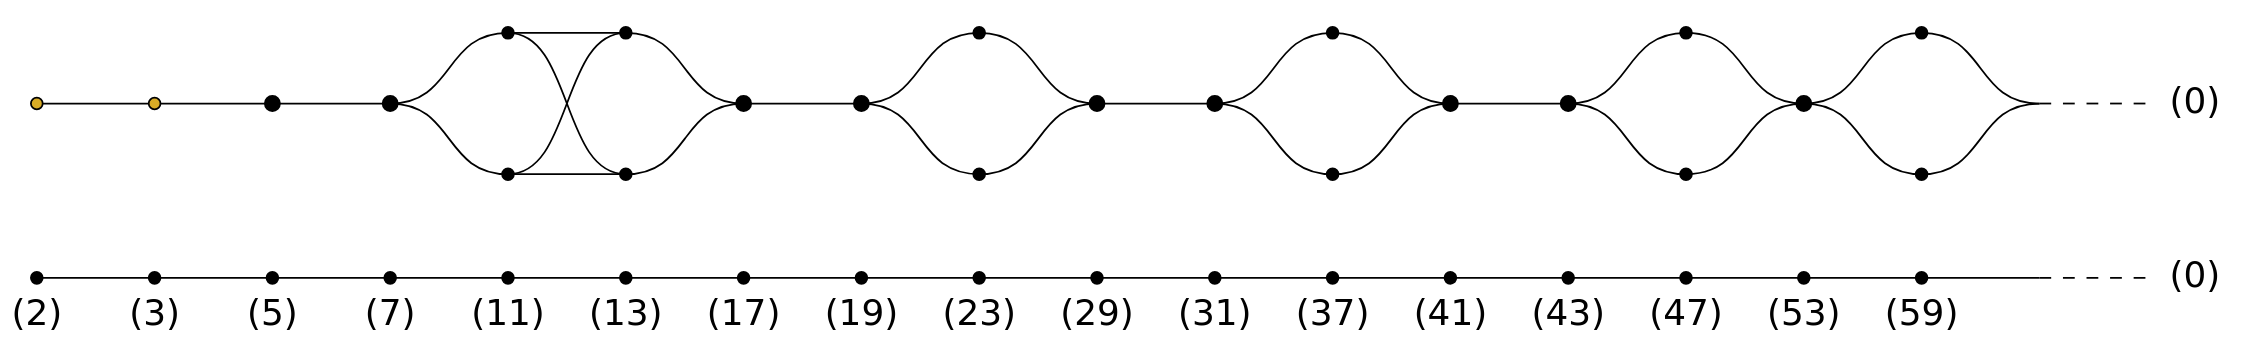
\includegraphics[width=0.7\textwidth]{Images/ramification_diagram_Zsqrt3.png}
			\caption{$\Spec(\Z[\!\sqrt{3}])\epi\Spec(\Z)$, per the \href{https://www.lmfdb.org/NumberField/2.2.12.1}{LMFDB}.}
			\label{fig:SpecZsqrt3_over_SpecZ}
		\end{figure}
		The behaviour of different points fall into three classes, all depicted differently in this diagram:
		\begin{itemize}
			\item \textbf{A single, black point} above a point $(p)$ of $\Spec(\Z)$ corresponds to the ideal $p\Z[\!\sqrt{3}]$ being a prime ideal of $\Z[\sqrt{3}]$, as we see with e.g. $(17)$. This point $17\Z[\!\sqrt{3}]$ of $\Spec(\Z[\!\sqrt{3}])$ is a \bemph{reduced point}, i.e. a point with multiplicity 1. In the number theory lingo, we say that $17$ is \bemph{inert} in the extension $\Q(\!\sqrt{3})/\Q$;
			\item \textbf{Two different black points} above a point $(p)$ of $\Spec(\Z)$ corresponds to the ideal $p\Z[\!\sqrt{3}]$ decomposing as a product of two distinct prime ideals $\Prid_1, \Prid_2$ in $\Z[\sqrt{3}]$ each with multiplicity 1, as we see with e.g. $(11)$ decomposing in $\Z[\!\sqrt{3}]$ as $(1-2\sqrt{3})(1+2\sqrt{3})$. Both of these points $\Prid_1, \Prid_2$ above $(p)$ are again reduced points of $\Spec(\Z[\!\sqrt{3}])$. In the number theory lingo, we say that $11$ is \bemph{completely split} in $\Q(\!\sqrt{3})/\Q$, and we say that $(1-2\sqrt{3})$ and $(1+2\sqrt{3})$ are the primes \bemph{above} $11$;
			\item \textbf{A single, yellow point} above a point $(p)$ of $\Spec(\Z)$ corresponds to the ideal $p\Z[\!\sqrt{3}]$ being the square\footnote{...or more generally, a power of a single prime ideal.} of a single prime ideal $\Prid$ in $\Z[\!\sqrt{3}]$, as we see with e.g. $3\Z[\!\sqrt{3}] = (\sqrt{3})^2$. This point $(\sqrt{3})$ is a \bemph{non-reduced point} of multiplicity 2. In the number theory lingo, we see that $3$ is \bemph{totally ramified} in $\Q(\!\sqrt{3})/\Q$, and we say that $(\sqrt{3})$ is the prime above $3$.
		\end{itemize}
	\end{enumerate}
\end{eg}




% talk about Diego's ramification intuition in the morphisms-y bit 		% section 2 	-- schemes + morphisms

	% appendices
	\section{A little bit about sheaves}
\label{appendix:A_sheaves}
The notion of a \emph{sheaf} is extremely important to scheme theory, and allows us to talk about local properties in an organised way. If you've never seen anything about them, I'll try to introduce them as best as I can.

\begin{eg}
	The main motivating example for a sheaf is the notion of sections of a continuous map $f:X \to Y$, that is, continuous maps $s:Y \to X$ such that $f \circ s = \id_X$. While not every continuous map admits such a continuous section, it is more likely that admit a \emph{local} section, i.e. there is an open $U \subseteq X$ and some continuous $s : U \to Y$ such that $f \circ s = \id_U$. For each open set $U \subseteq X$, we will write $\ints_f (U)$ for the set of local sections of $f$ at $U$. Then we notice some important properties:
	\begin{itemize}
		\item \textbf{Restriction:} if $U \supseteq V$ and $s \in \ints_f(U)$ is a local section at $U$, then the restriction $s|_V$ is a local section at $V$, i.e. $s|_V \in \ints_f(V)$;
		\item \textbf{Locality:} if $U = \bigcup_i U_i$ and two sections $s,t \in \ints_f(U)$ agree on each $U_i$ (i.e. $s|_{U_i} = t|_{U_i}$ for each $i$), then they must agree on all of $U$, $s=t$. That is to say, sections are fully determined by their restrictions;
		\item \textbf{Gluing:} if $U = \bigcup_i U_i$ and for each $i$ we have a section $s_i \in \ints_f(U_i)$ which agree on overlaps (i.e. such that $s_i|_{U_i \cap U_j} = s_j|_{U_i \cap U_j}$ whenever $U_i \cap U_j \neq \varnothing$). That is to say, we may glue together compatible sections.
	\end{itemize}
	This local-global structure is exactly the kind of thing that sheaves are meant to capture.
\end{eg}

\begin{defn}
	Let $X$ be a topological space. A \bemph{presheaf of sets} (respectively, of abelian groups, of rings, etc.) on $X$ is an assignment of a set (resp. abelian group, ring, etc.) $\mathcal{F}(U)$ to each open set $U \subseteq X$, along with a function (resp. homomorphism, morphism, etc.) $\rho^U_V : \mathcal{F}(U) \to \mathcal{F}(V)$ whenever $U \supseteq V$ which `behave like restriction maps', i.e. $\rho^U_U = \id_U$ and $\rho^V_W \circ \rho^U_V = \rho^U_W$ for each tower $U \supseteq V \supseteq W$. An element $s \in \mathcal{F}(U)$ is called a \bemph{section} of $\mathcal{F}$ at $U$, and for $U=X$ a section $s \in \mathcal{F}(X)$ is called a \bemph{global section}. A presheaf $(\mathcal{F}, \rho)$ is said to be a \bemph{sheaf} if:
	\begin{itemize}
		\item[(L)] for each open cover $U = \bigcup_i U_i$, two sections $s,t \in \mathcal{F}(U)$ are equal if and only if $\rho^U_{U_i}(s) = \rho^U_{U_i}(t)$ for each $i$; and
		\item[(G)] for each open cover $U = \bigcup_i U_i$ and family of sections $\{s_i \in \mathcal{F}(U_i)\}_i$ such that
			\[
				\rho^{U_i}_{U_i \cap U_j}(s_i) = \rho^{U_j}_{U_i \cap U_j}(s_j), \qquad U_i \cap U_j \neq \varnothing,
			\]
			there is a section $s \in \mathcal{F}(U)$ such that $s_i = \rho^U_{U_i}(s)$.
	\end{itemize}
\end{defn}

As before, property (L) just says that sections are fully determined by their restrictions, and property (G) just says that we can glue sections together. 

\begin{eg}
	\begin{enumerate}[(i)]
		\item As before, $\ints_f$ defines a sheaf of sets on $X$;
		\item The assignment $\mathcal{F} = \mathrm{Map}(-, \R)$ on open sets of $X$, where $\mathrm{Map}(U, \R)$ denotes the $\R$-algebra of continuous maps $U \to \R$, is a presheaf of $\R$-algebras with $\rho^U_V(f) := f|_V$. Definition of equality of functions tells us that $\mathcal{F}$ satisfies property (L), and the gluing lemma ensures that it satisfies property (G). Thus, $\mathcal{F}$ defines a sheaf on $X$;
		\item \textbf{Non-example:} The assignment $\mathrm{Map}_{\mathrm{bdd}}(-, \R)$ of bounded continuous functions still defines a presheaf with usual restrictions, and this presheaf satisfies property (L). However, we do not necessarily have property (G), since for example the function $\id_\R : \R \to \R$ is unbounded and continuous, but with respect to the open cover $\R = \bigcup_{n \in \Z} (n-1, n+1)$, its local sections are all bounded. These restrictions thus do not glue to a bounded function;
		\item \textbf{Non-example:} We may define a presheaf $\underline{\Z}$ of commutative rings on any topological space $X$ by assigning $\underline{\Z}(U) := \Z$ and $\rho^U_V = \id_{\Z}$. Any section of $\underline{\Z}$ is just an integer, so if we take two disjoint opens $U, V$, then the sections $1 \in \underline{\Z}(U), 2 \in \underline{\Z}(V)$ do not glue to a section on $U\cup V$. This is called the \bemph{constant presheaf} associated to $\Z$;
		\item We may instead define the presheaf $(\underline{\Z})^+$ the assign to each $U$ the set of locally constant functions $U \to \Z$. Then we find that we do, indeed, have properties (L) and (G), so this does define a sheaf of commutative rings on $X$. This is called the \bemph{constant sheaf} associated to $\Z$.
	\end{enumerate}
\end{eg}

% morphisms of sheaves
% stalks of sheaves % stalk(F) = colim_U F(U)
% (locally) ringed spaces & their morphisms 	% appendix A 	-- sheaves
\end{document}
